%! TEX root = 'main.tex'

\section{Design}
\label{sec:design}

In this section, we present the design of our project. It has two major parts, the main module setups SMAP environment, monitors kernel to user space accesses, intercepts and handles related page faults and makes the page attributes transitioning. The other part is the hypervisor. As briefly mentioned in the introduction, the hypervisor in charges of isolating the SMAP feature to certain processes.

\subsection{Monitoring Kernel to User Space Accesses}

This is the major issue we faced when addressing kernel TOCTOU vulnerability. Reading and writing memory is the most common operation that a computer system does. So even with virtualization technology, there is no trap event on accessing memory. However, what makes the kernel TOCTOU vulnerability special is the fact that it's always the case that the kernel accesses user space. So we employ SMAP to monitor such behavior. 

Because there is no reasons for the user parameters to change during the ongoing syscall, we should make them unchangeable. For now, due to the practical reason that SMAP works on page granularity, we protect all the pages that contain the user parameters from being tampered with. Conflicts caused by this will be solved later in this section.

As mentioned earlier, once SMAP enabled, kernel accessing user space triggers page fault exceptions, so we intercepts OS's page fault handler. But the handler needs to handle all the exceptions in the system, it's a efficiency critical component. So the first thing we need to do is to distinguish the ones that caused by SMAP or by our subsequent protection. Notice that SMAP is a very strict rule. For example, in Linux system, the two user-data-access functions copy\_to\_user() and copy\_from\_user() temporarily disable SMAP right before accessing user space and re-enable it right after. That means the system should not seen any SMAP caused exception. Once there is one, the Linux kernel will take it as a serious error, then panic. The same with Windows, it didn't support SMAP yet, it also crashes when sees such exceptions.

Even though Intel provides two new instructions CLAC/STAC to temporarily disable/enable the feature, in page fault handler, it's already too late to cancel it.

Now we have a efficient hardware mechanism that can inform us whenever there is a kernel-to-user access. The rest is to protect the pages and to let the system continue. We choose to put the faulting page into the kernel space by setting the attributes in theirs page table entries(PTE). By doing so, the page fault exception is handled because it's no longer kernel accessing a user page, also the faulting page is protected from other user threads. 

\subsection{Page Attribute Transition} % transition or conversion? Or something else?


The memory management unit(MMU) in x86 architecture use page tables to map between virtual and physical pages~\cite{intelpaging}. Every page in the virtual memory has corresponding page table entries. As shown in~\autoref{fig:pte}, it contains bits that describes the page. For example, whether a page belongs to kernel or user depends on the 'User/Supervisor' bit. If the bit is set, then this page is a user page; if not, it's a kernel page. Obviously, user pages can be accessed by both user code and kernel code, but kernel pages can only be accessed by kernel code. 

\begin{figure}[th]
  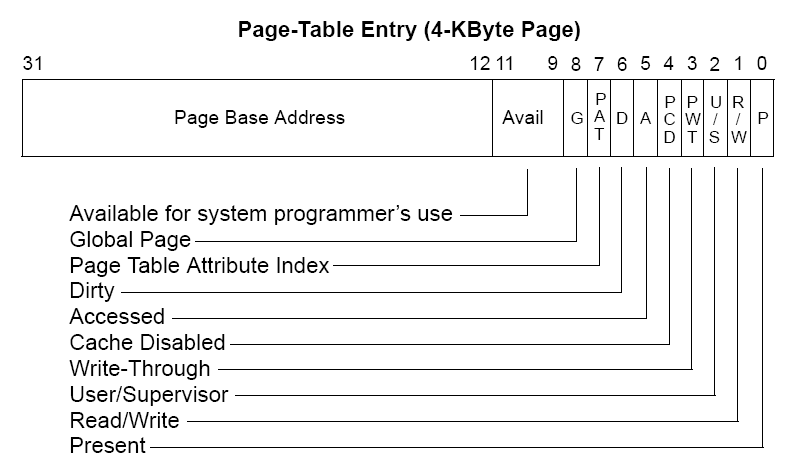
\includegraphics[width=0.47\textwidth]{figures/pte}
  \centering
  \caption{U/S, the 'User/Supervisor' bit, controls access to the page based on privilege level. If the bit is set, then this page is considered in user mode space and be accessed by all code; if the bit is not set, then it's considered in kernel mode space and can be accessed only by kernel mode code. }
  \label{fig:pte}
\end{figure}


When handling a page fault exception, the faulting virtual address is always stored in the CR2 register and the root of the current process's page tables is stored in CR3 register. First we need to walk through the page table to locate the corresponding page table entry of the faulting address. Then to put a user page into kernel space, simply changes the 'U/S' bit to 0. It becomes a kernel page even thought it's address doesn't look so, because normally on x86 Windows system, the kernel space is above address 0x80000000. We also can change it back by doing the opposite with the 'U/S' bit. We do so when the current syscall ends.

When the page is in kernel space, it's protected from user code accesses, as shown in~\autoref{fig:denyuserwrite}.

\begin{figure}[th]
  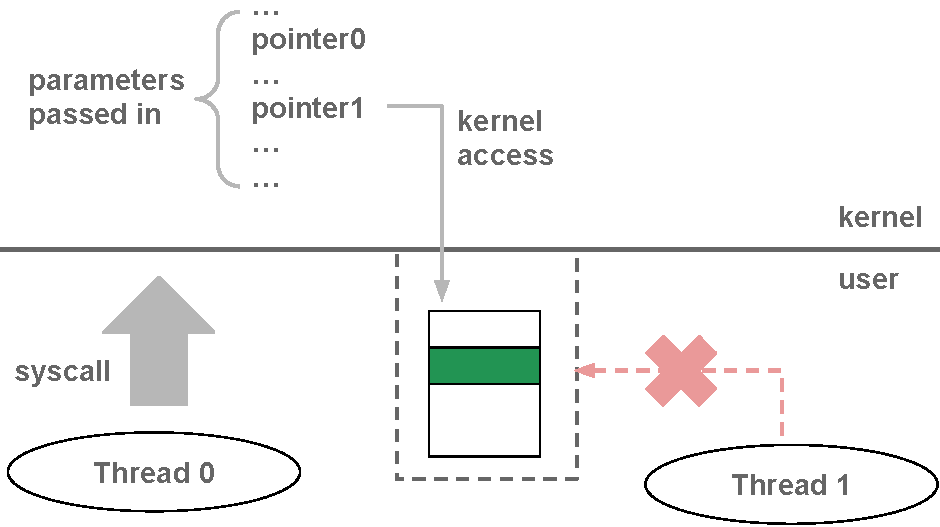
\includegraphics[width=0.47\textwidth]{figures/denyuserwrite}
  \centering
  \caption{}
  \label{fig:denyuserwrite}
\end{figure}


This is the base of our model. In reality, it's common that other user threads try to access data within the same page. For example, global variables or heap data when threads share the same heap pool. Even there are cases where read-only data is merged into one section with code by the compiler. We need to handle these situations as well.

To address this issue, user reading and user writing should be treated separately. Because reading doesn't change any data, it's safe to our mitigation. So when reading happens, we changes the page back to user space in order to fulfill the request. But we still want to remain its protection, because once we put it back, before another kernel access, this page is subject to any user access including writing. The solution is setting the page as read-only as well so subsequent writing triggers exception too. Certainly we record those information so when handling write violation we could behave accordingly and later restore the page attribute correctly. ~\autoref{fig:pagestate} shows the transitions due to different causes. 


\begin{figure}[th]
  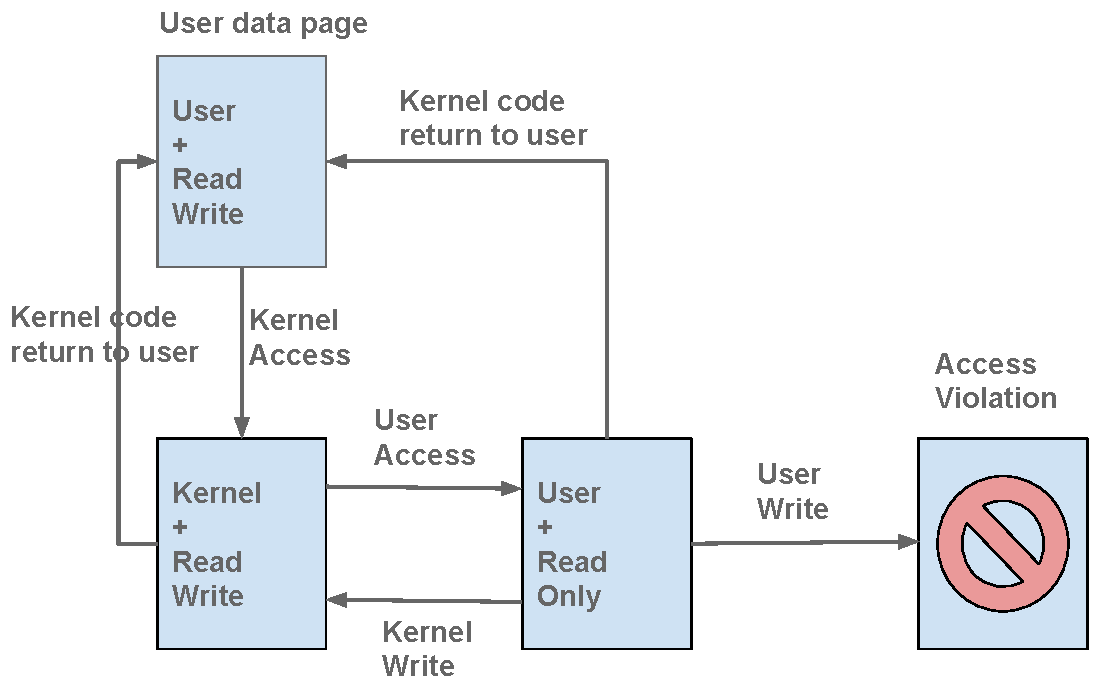
\includegraphics[width=0.45\textwidth]{figures/pagestate}
  \centering
  \caption{Page attributes transit between kernel mode and user mode. When kernel mode code ends, for example, system service returns to user mode, the page will be set back to the original permission}
  \label{fig:pagestate}
\end{figure}


Kernel reads/writes and user reads make the page transit from spaces and change attributes. The challenge remain is to handle user writes. 


\subsection{Solving Write Conflict }
Subject to the x86 architecture, the hardware mechanism works only on page granularity.

For practical mitigations, compatibility is important. There are cases that program writes shared data or writes the data of the same page. Under the protection we just mentioned, such write access will trigger a page fault and causes thread exit. No synchronizing mechanism for shared resource, for example, user memory which is the root cause of kernel TOCTOU vulnerability. 

Since pages only be protected during the current system call, our solution is to hold the write thread, waiting for the system call to end. "Hold" means the write thread will give up it's time slice, letting operating system re-scheduling. 

\begin{figure}[th]
  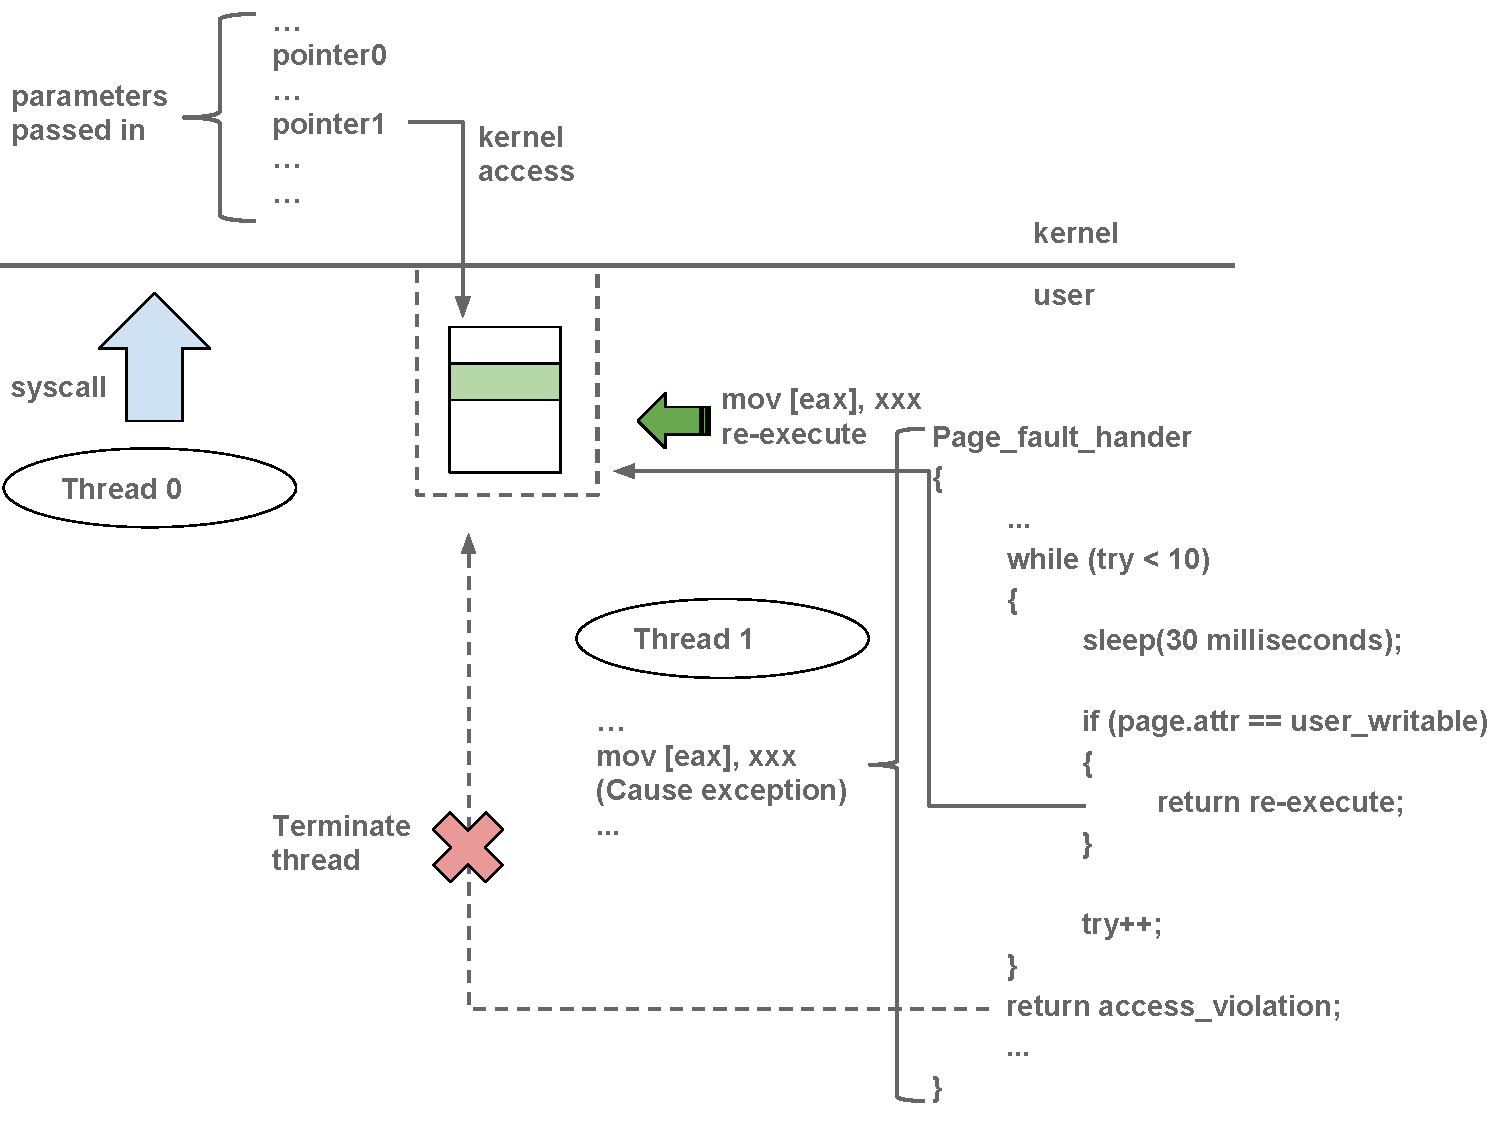
\includegraphics[width=0.47\textwidth]{figures/reexecute}
  \centering
  \caption{}
  \label{fig:reexecute}
\end{figure}

As shown in~\autoref{fig:reexecute}, Thread 1 is trying to access a protected page. Instead of terminating it, we hold it in the context of page fault exception, specifically, calling KeDelayExecutionThread() to put it to "sleep". But only for a certain amount of time, then it checks whether the page now is writable. If so, the page fault handler finish this exception and re-execute the fault instruction, otherwise, it waits for another round. A threshold is set to prevent infinite waiting. For example, after ten times, the thread will be terminated.

\subsubsection{Differences between Exception and Interruption}

To explain why thread can wait in the context of page fault exception, we briefly review the difference between exception and interruption of x86 architecture.

In x86 architecture, external(hardware) interrupts, software interrupts and exceptions are all handled through the interrupt descriptor table (IDT). 

External interrupt is a signal from a device such as network card, keyboards, telling CPU that an event just happened, need CPU to handle it immediately. External interrupts from different devices have different priorities, but mostly they have a higher priority than operating system thread scheduler. Meaning operating system need to handle external interrupt before any user-mode program, even most of the kernel code. To put the processor wait inside an external interrupt handler is not a good  practice, it extremely affects system performance. Operating system finishes external interrupts as soon as possible, even the lengthy low-priority part of a task is deferred for later execution. For example, in Windows operating system such mechanism is called DPC(Deferred Procedure Call). A single long-running deferred procedure call will be detected and raise a BugCheck (DPC\_WATCHDOG\_VIOLATION). DPCs should not run longer than 100 microseconds and ISRs should not run longer than 25 microseconds~\cite{msdnwatchdog}. In such environment, thread scheduling is not feasible.

Software Interrupt is an interrupt that signaled by software using "INT" instruction, such as "INT 0x2e", "INT 0x80" for system calls. 

What we leveraged in this project is exceptions. Exception is generated internally by the CPU to let the operating system handling an event or error such as double fault, page fault, general protection fault, etc. Different than external interruption, the priority of the exception handler is the same as the code that triggers the exception. Priority, in Windows operating system's term, is IRQL(Interrupt Request Level). When a user-mode program triggers a page fault exception, the control flow will be immediately transferred to the page fault handler which resides in the kernel, but the it's IRQL still stay at PASSIVE\_LEVEL which is the level where user program runs. Under PASSIVE\_LEVEL, thread scheduling is feasible.

\subsection{Releasing Protected Pages}

When a system call ends, all the related pages that being protected should be released. Their attributes will be restored which set free other waiting threads. There original attributes are recorded not only for restore purpose but also used as ground truth when to decide how to handle a page fault.


\begin{comment}
\begin{figure}[th]
  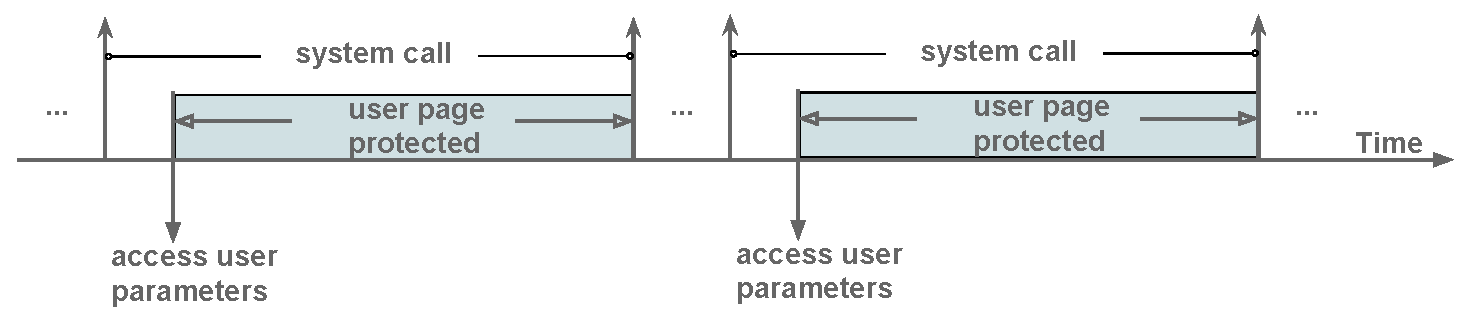
\includegraphics[width=0.47\textwidth]{figures/timeline}
  \centering
  \caption{The page protection period is within one system call cycle, this is based on the fact that kernel TOCTOU vulnerability does not happen across system calls.}
  \label{fig:timeline}
\end{figure}
\end{comment}


%We choose to install a hook near the end of system calls. On Windows operating system, such place could be, for example, KiServiceExit. Because during this function, Windows OS delivers pending APC~\cite{apc} which also needs to access user data. The hooking point that we choose is right after it calls KiDeliverAPC. It's not the very last instruction that the kernel mode execute, but we consider it close enough to the end of a system call.


Protected pages should be released according to specific thread. Meaning, when one thread finishes a system call, only those pages that related to itself should be released. To distinguish different thread in a process, TEB (Thread Environment Block~\cite{teb}) could be used as an identifier. TEB describes the state of a thread. Each thread has its own TEB structure and it's address can be found through segment register FS (at FS:0x18) which points to different locations for each thread. 

\subsection{Hypervisor}

SMAP is a system wide feature. Due to the way Windows kernel retrieve user-mode parameters (continuous read of one buffer may even cause a series of exceptions), huge amount of exception is expected. Also, SMAP caused exception needs proper handling, it can't be passed to operating system. Moreover, page fault is one of the core mechanism that builds up MMU of x86 architecture. Its handler is highly optimized to handle tremendous amount of exceptions, even a few more instructions introduced may affect system's performance.  To eliminate unnecessary system overhead, we provide a thin hypervisor that only enables SMAP on certain processes.

Not all the processes need to be monitored, such as the ones that already run with administrator or system privilege. Because kernel TOCTOU vulnerabilities are mostly used to escalate privilege. Normally, services that may potentially be controlled locally or remotely by attackers and alien processes are the suspects of privilege escalation attacks.

The hypervisor is simple and efficient. It's loaded as a Windows kernel driver at runtime, so the operating system doesn't need to change the way it boots. It only lifts the running operating system into VMM guest mode in order to intercept system events and change system's behavior. No hardware emulation is needed.  

\subsubsection{Process Context Switch}

One of the main character of virtual memory of x86 architecture is that each process has its own virtual address space which shared by multiple threads that exist within a process. Each process has a private set of page tables that represents the mappings between virtual memory and physical memory. Their root is stored in control register CR3. 

In Windows operating system, instead of process, thread is the base unit for task scheduling. But when scheduling to a thread of another process, the virtual address space needs to change too. Hence the changing of CR3 can be the indicator for process context switch. Fortunately, Intel's virtualizaton technology is able to capture the event.


\subsubsection{Virtualization Techniques}

"MOV from/to CR3" is one of the instructions that cause VM exits when they are executed in VMX non-root operation(guest mode). For example, "MOV CR3, EAX", where general register EAX contains the new page directory address, indicates an on going process context switch.

Our hypervisor handles VM exits and compare the new CR3 value with the ones that need to be monitored. If match, it sets the SMAP bit in the CR4 of VMCS(Virtual Machine Control Structure) so that when the VM resumes, the new value can be updated to the processor's CR4. Correspondingly, when the monitored processes are switched out, hypervisor does the opposite, clearing the SMAP bit. In such a way, the SMAP feature is only enabled in certain processes, as shown in~\autoref{fig:processmap}.

\begin{figure}[th]
  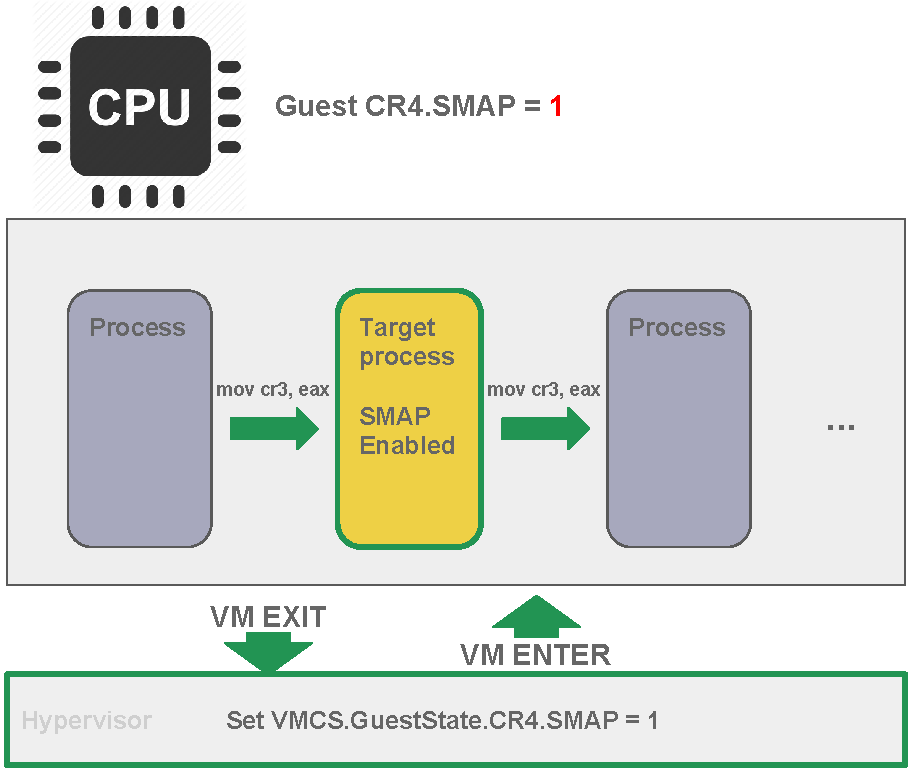
\includegraphics[width=0.47\textwidth]{figures/processmap}
  \centering
  \caption{SMAP is only enabled on the target process. In other words, only target process can trigger SMAP exceptions.}
  \label{fig:processmap}
\end{figure}
